\begin{problem}
什么是数据仓库,其四大特色是什么?
\end{problem}

\begin{solution}
数据仓库就是一个面向主题的、集成的、非易失(稳定的)、随时间不断变化的数据集合,用于支持经营管理过程中决策制定。

数据仓库四大特色:
\begin{enumerate}[label=\arabic*.]
    \item 面向主题:指数据仓库内的信息是按主题进行组织的,为按主题进行决策的过程提供信息。(数据仓库中无法做到面向应用:没有办法模拟出所有的决策)
    \item 集成:数据仓库中的数据是为分析服务的,而分析需要多种广泛的不同数据源以便进行比较、鉴别,因此数据仓库中的数据必须从多个数据源中获取,这些数据源包括多种类型数据库、文件系统以及Internet网上数据等,它们通过数据集成而形成数据仓库中的数据
    \item 非易失(稳定):数据仓库中的数据是经过抽取而形成的分析型数据,不具有原始性,主要供企业决策分析之用,执行的主要是“查询”操作,一般情况下不执行“更新”操作。同时,一个稳定的数据环境也有利于数据分析操作和决策的制订
    \item 随时间不断变化:企业不仅仅关心某一个时间节点的情况。数据仓库的数据通常带有时间属性,同时必须以一定时间段为单位进行统一更新。
\end{enumerate}
\end{solution}


\begin{problem}
为什么在传统的以数据库为核心的事务处理环境中不适宜建立DSS等分析型应用?
\end{problem}

\begin{solution}
\vspace{-0.7em}
\begin{multicols}{2}
    \begin{enumerate}[label=\arabic*.]
        \item 事务处理和分析处理的性能特性不同
        \item 数据集成问题
        \item 数据的动态集成问题
        \item 历史数据问题
        \item 数据的综合问题
        \item 数据的访问问题
    \end{enumerate}
\end{multicols}
\vspace{-0.7em}
\end{solution}


\begin{problem}
什么是数据仓库中的粒度?为何要在数据仓库中采用多重粒度?试举例说明。
\end{problem}

\begin{solution}
粒度是对数据仓库中的数据的综合程度的一个度量,既影响数据仓库中数据量的多少,也影响数据仓库能够回答询问的种类。

采用多重粒度是为了应对不同级别的粒度要求:对于大粒度数据,需要快速存储设备并提高性能;对于小粒度数据,需要低速存储设备并满足细节查询。

\begin{figure}[H]
	\setcounter{subfigure}{0}
	\centering
	\vspace{-1em}	
	\subfloat[高粒度、低细节的数据无法应对过于细节的问题]{
	\begin{minipage}[t]{0.6\linewidth}
	\centering
	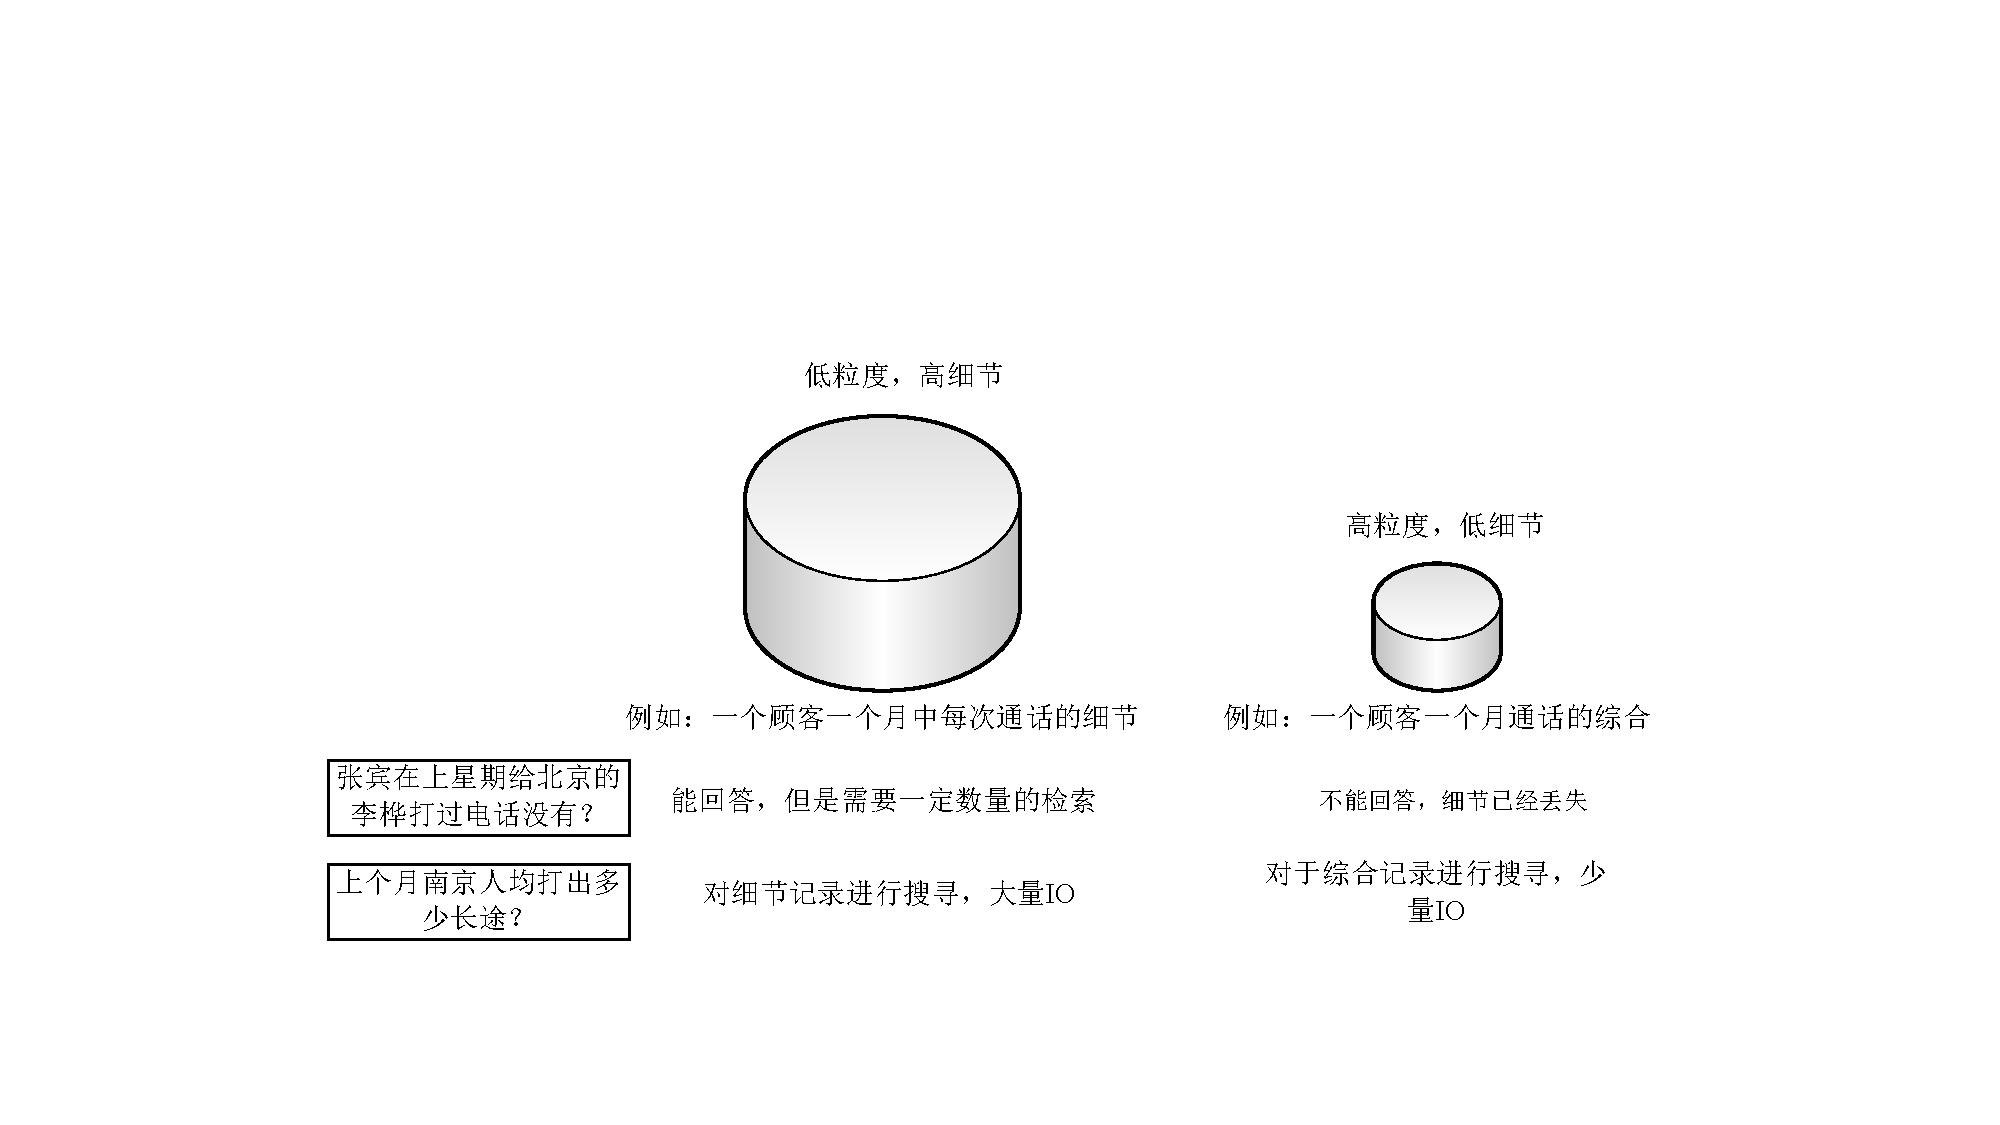
\includegraphics[width=0.97\linewidth]{images/多重粒度举例1.pdf}
	\end{minipage}
	}
	\subfloat[无论是高粒度还是低粒度的数据都可以应对]{
	\begin{minipage}[t]{0.37\linewidth}
	\centering
	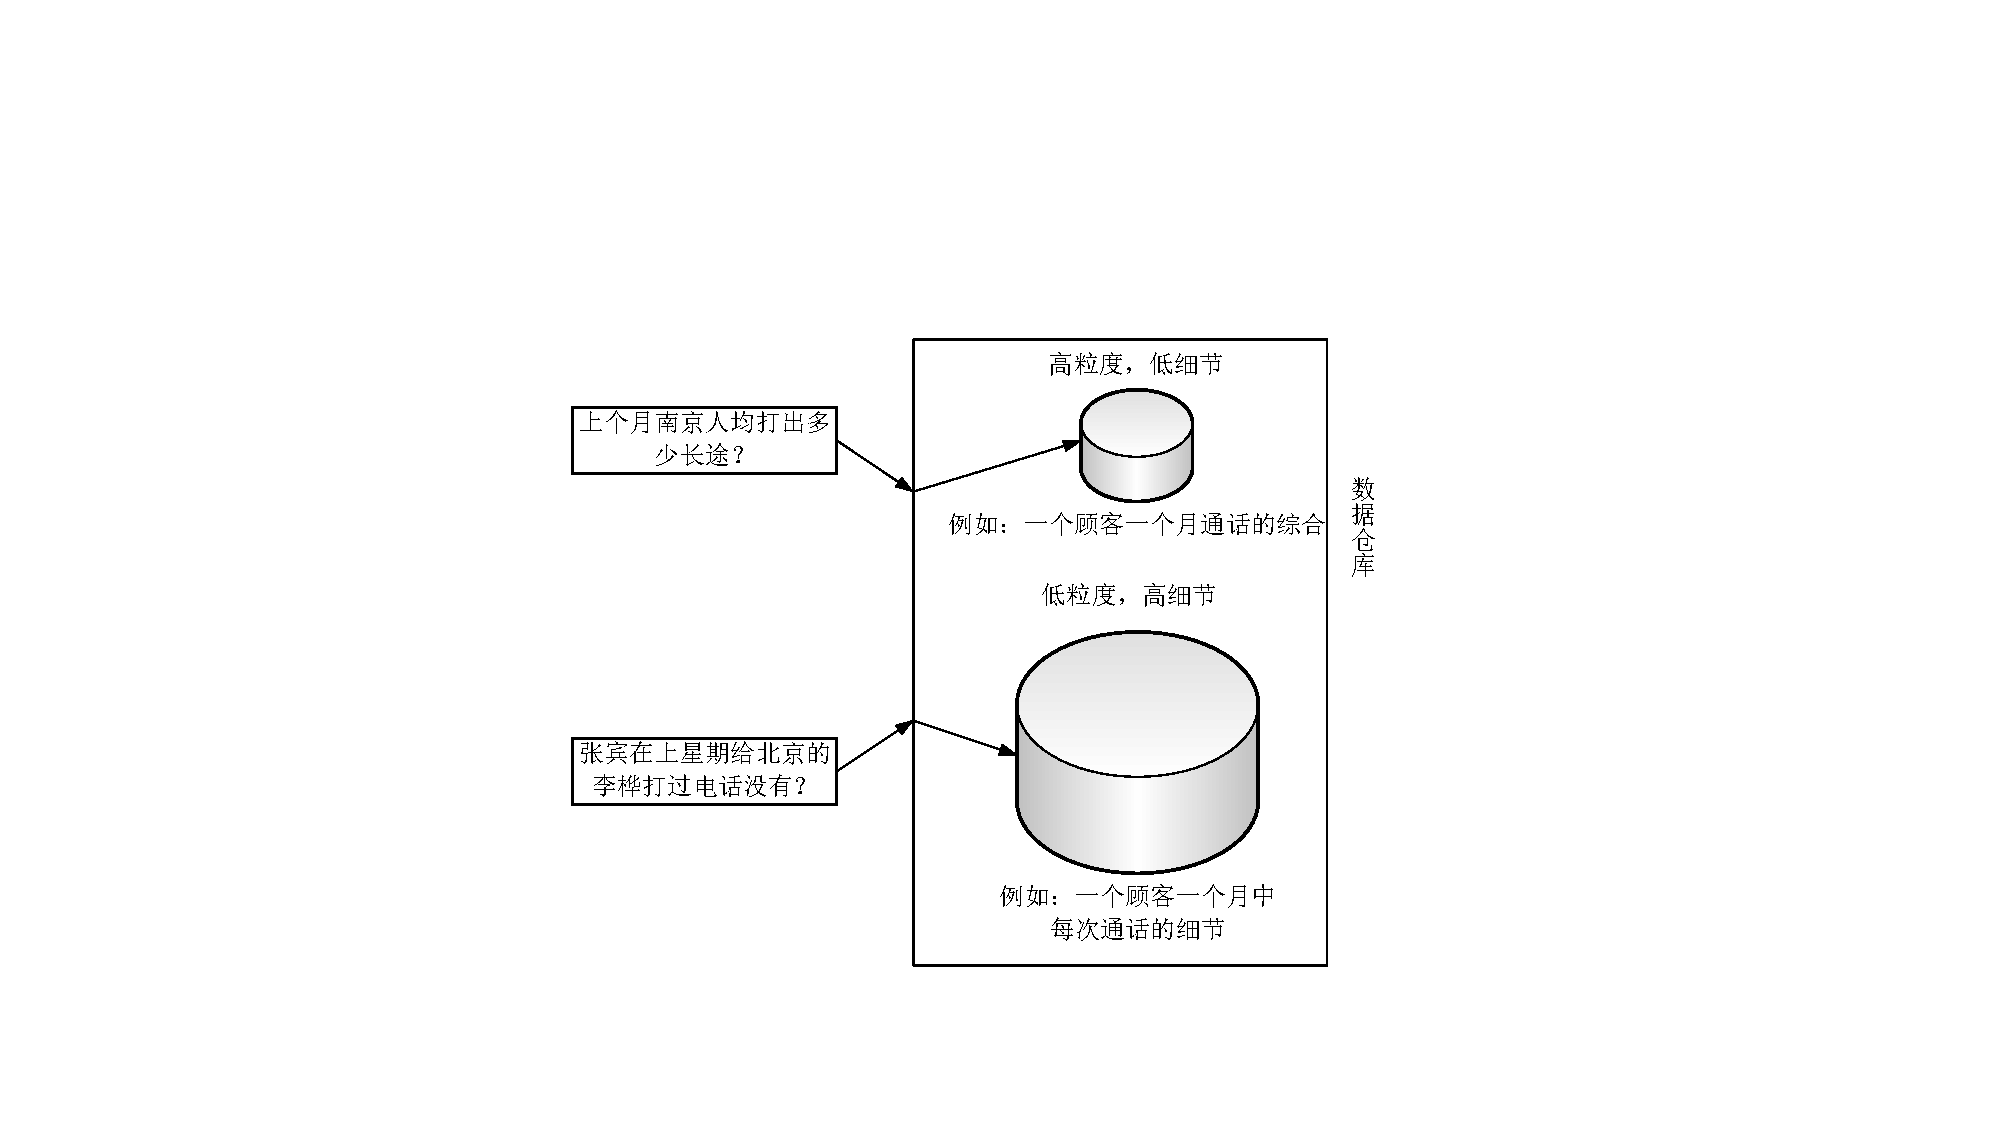
\includegraphics[width=0.97\linewidth]{images/多重粒度举例2.pdf}
	\end{minipage}
	}
	\centering
	\vspace{-1.5em}
\end{figure}

\end{solution}


\begin{problem}
数据仓库的物理模型设计优化技术有哪些?对这些技术进行简要的说明。
\end{problem}

\begin{solution}
常用的一些技术有:合并表、建立数据序列、引入冗余、表的物理分割、生成导出数据和建立广义索引。
\begin{itemize}
    \item 合并表:在常见的一些分析处理操作中,可能需要执行多表连接操作。为了节省I/O开销,可以把这些表中的记录混合存放在一起,以减低表的连接操作的代价。
    \item 建立数据序列:根据周期运行的数据分析应用访问数据的先后顺序,维护一个冗余的序列,提前把需要的数据按需准备好,在需要访问的时候就不再需要访问不同的表格中的不同元组,从而提升效率。
    \item 引入冗余:在面向某个主题的分析过程中,通常需要访问不同表中的多个属性,而每个属性又可能参与多个不同主题的分析过程。因此可以通过修改关系模式把某些属性复制到多个不同的主题表中去,从而减少一次分析过程需要访问的表的数量。
    \item 表的物理分割:可以根据表中每个属性数据的访问频率和稳定性程度对表的存储结构进行分割。
    \begin{itemize}
        \item 对于访问频率较高的属性,可以单独考虑其物理存储组织,以便选择合适的索引策略和特定的物理组织方式。
        \item 对于需要频繁更新的属性,也可以单独组织其物理存储,以免因数据更新而带来的空间重组、重构等工作。
    \end{itemize}
    \item 生成导出数据:在原始、细节数据的基础上进行一些统计和计算,生成导出数据,并保存在数据仓库中。
    \item 广义索引:用于记录数据仓库中数据与“最”有关的统计结果的索引被称为“广义索引”。(例如当月销售额最高的商店)
\end{itemize}
\end{solution}


\begin{problem}
什么是数据仓库中的历史完整性/一致性?为保持历史完整性/一致性,可以采用哪些方式?试举例说明。
\end{problem}

\begin{solution}
历史完整性:部分维度属性是会随时间而发生变化的,若只是将这些变化的维度属性值作简单的修正,即在维度表中只保留该维度属性的当前值,这会直接影响到对事实表中该维度属性所对应的事实数据元组的访问,特别是无法根据维度属性值的变化情况来进行分析处理。历史完整性是保证维度中的历史数据在改变之后不丢失。

针对渐变维度(商品表)的方法
\begin{itemize}
    \item 改写属性值(类型1):容易实现,但不能对旧属性值的任何历史数据进行维护(无法保证历史一致性)
    \item 添加维度行(类型2):准确跟踪渐变属性的主要方法,也是跟踪历史变化的最常用的方式;引入新的行用来反映新的属性值;增加了维度行的膨胀;可以引入生效或截止日期
    \item 添加维度列(类型6):使用维度列保存旧的属性值;不适合跟踪维度属性大量变化
    \item 类型6\ ($1+2+3$)
\end{itemize}

\begin{figure}[H]
    \centering
    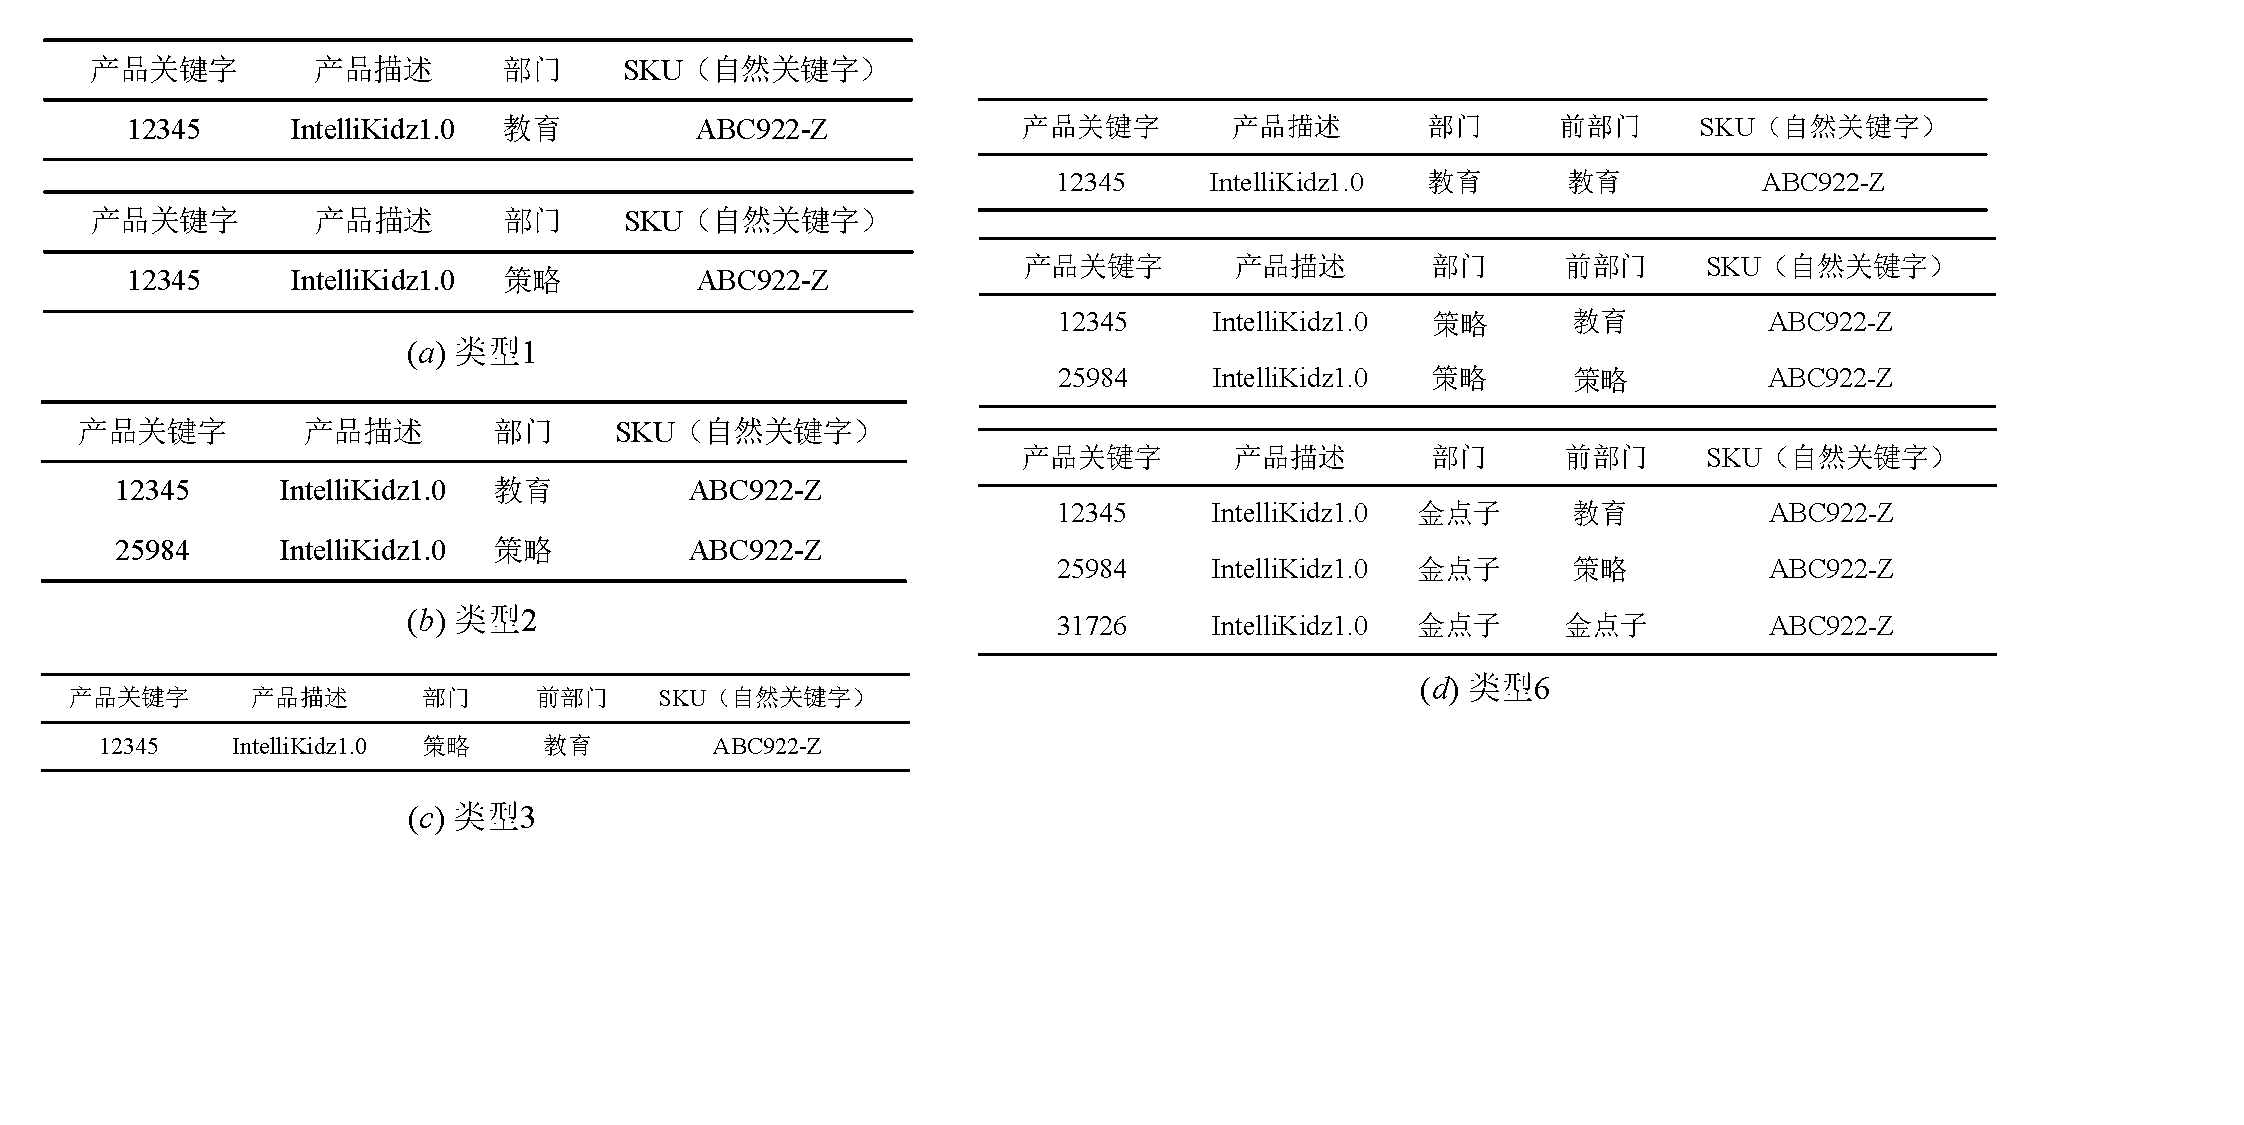
\includegraphics[width=\textwidth]{images/类型1,2,3,6.pdf}
    \vspace{-1em}
\end{figure}

针对快变维度的方法
\begin{itemize}
    \item 微型维度:将分析频率高或变化频率大的属性拆成为独立的微型维度。例如客户维度中的年龄,性别,收入水平等属性,它们的每一种取值组合构成微型维度表中的一行。
    \item 预设波段:对于诸如收入与购买总额等不断变化的属性,应该被转换成呈波段分布的范围,即进行离散化处理,使其只能在数目相当小的离散值中取值,以减少维度表中的数据量。
\end{itemize}

\end{solution}


\begin{problem}
简述数据仓库刷新的方法,并对每一种方法进行简单的说明。
\end{problem}

\begin{solution}
一般数据刷新的方法包括:时间戳、DELTA文件、建立映象文件和日志文件。

\begin{spacing}{1.2}
    \centering
    \begin{longtable}{|m{1.2cm}<{\centering}|m{4.7cm}|m{4.7cm}|m{3.3cm}|}
        \hline
        方法      & \multicolumn{1}{c|}{适用情况/实现方法}                                                               & \multicolumn{1}{c|}{优点}                                                         & \multicolumn{1}{c|}{缺点}                             \\ \hline
        时间戳     & 若数据库中的记录有时间属性,则可根据OLTP数据库中的数据有无更新,以及在执行更新操作时数据的修改时间标志来实现数据仓库中数据的动态刷新。   &                                                            & 大多数数据库系统中的数据并不含有时间属性。          \\ \hline
        DELTA文件 & 有些基于OLTP数据库的操作型应用程序在工作过程中会形成一些DELTA文件以记录该应用所作的数据修改操作,可根据该DELTA文件进行数据刷新。 & 采用此方法可避免对整个数据库的对比扫描,具有较高的刷新效率。                             & 这样的应用程序并不普遍,修改现有的应用程序的工作量又太大。  \\ \hline
        建立映象文件  & 在上一次数据刷新后对数据库作一次快照;在本次刷新之前再对数据库作一次快照;比较两个快照的不同,从而确定数据仓库的数据刷新操作。         & 对于数据库和操作型应用无特别要求。                                          & 需要占用大量的系统资源;可能较大地影响原有数据库系统的性能。 \\ \hline
        日志文件    & 一般来说,现代OLTP数据库都有日志文件,可根据OLTP数据库的日志信息来实现数据仓库的数据刷新。                       & 日志是OLTP数据库的固有机制;不会影响原有OLTP数据库的性能;具有比DELTA文件和建立映象文件更高的刷新效率。 & 无法应用于无日志文件机制的遗留数据库系统等。         \\ \hline
    \end{longtable}
	\end{spacing}
\vspace{-0.5em}
\end{solution}


\begin{problem}
数据仓库中的ETL技术是什么?在数据仓库架构中ETL完成什么任务?
\end{problem}

\begin{solution}
ETL是用来描述将数据从来源端经过抽取(extract)、转换(transform)、加载(load)至目的端的过程。
\begin{itemize}
    \item 数据抽取:数据仓库中的数据来源于数据源,将数据源中数据通过网络进行抽取,并经加工、转换、综合后形成数据仓库中的数据,这就是数据仓库的数据抽取。
    \item 数据转换:数据元素的重命名、格式化,数据编码的转换(解析、校正、标准化、增补)
    \item 数据刷新
    \begin{itemize}
        \item 经过抽取进入数据仓库的数据,在经过一段时间后要重新修正,修改那些过时的数据,保存那些不变的数据,此种动作称为数据仓库的数据刷新。
        \item 数据刷新的过程与抽取类似,但刷新的数据量往往小于抽取的数据量。由于仅需要对修改过的数据进行刷新,因而其实现难度与复杂性要大于数据抽取。
    \end{itemize}
    \item 数据装载:数据经过转换、清洗后,需要装载到目标数据库中。数据装载的方式有多种:全表对比方式、时间戳方式、日志表的方式、全表删除后再插入的方式。
\end{itemize}

\begin{figure}[H]
    \centering
    \vspace{-0.2em}
    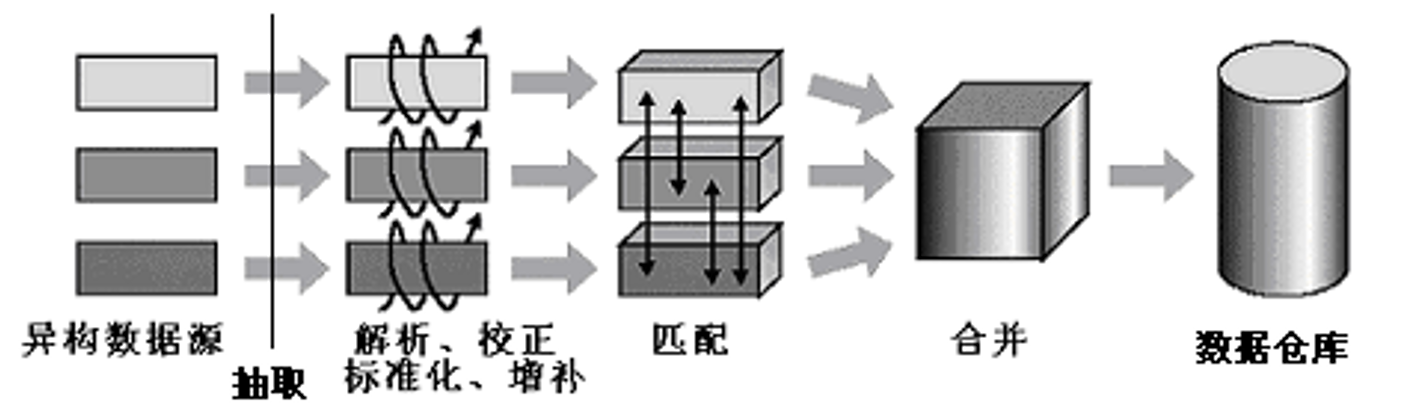
\includegraphics[width=0.6\textwidth]{images/ETL过程.png}
    \caption*{ETL过程}
    \vspace{-1.3em}
\end{figure}
\end{solution}


\begin{problem}
为什么在数据仓库体系中还需要建立数据集市?在企业中建立数据仓库和数据集市体系的方法主要有哪四种?请分别描述这些方法,并总结其优点和缺点。
\end{problem}

\begin{solution}
数据仓库与数据集市的关系类似于传统关系数据库系统中的基表与视图的关系。数据集市的数据来自数据仓库,它是数据仓库中数据的一个部分与局部,是一个数据的再抽取与组织的过程。

局性数据仓库往往太大,在实际应用中将它们按部门或个人分别建立反映各个子主题与区域的局部性数据组织,它们即是数据集市。因此,有时我们也称它为部门数据仓库;不同的主题会应用到的数据不同,对数据的时效性等部分要求不同。

\begin{figure}[H]
	\setcounter{subfigure}{0}
	\centering
	\vspace{-1em}	
	\subfloat[自顶向下的结构]{
	\begin{minipage}[t]{0.48\linewidth}
	\centering
	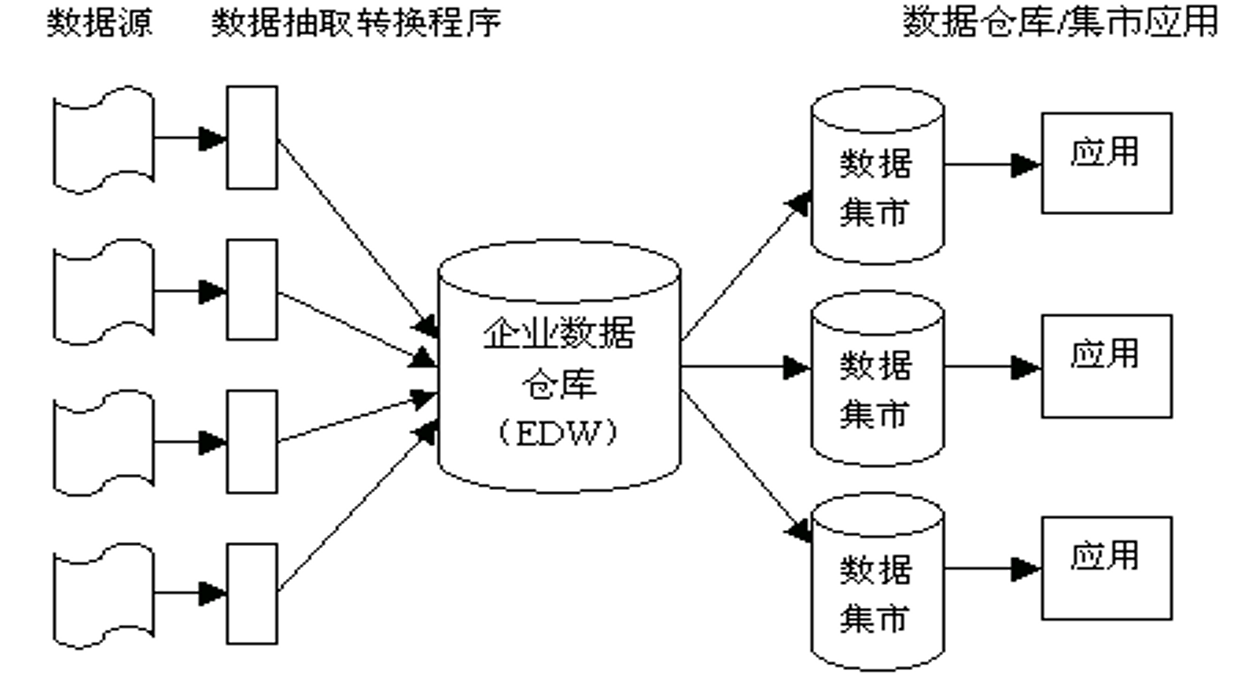
\includegraphics[width=0.97\linewidth]{images/自顶向下的结构.png}
	\end{minipage}
	}
	\subfloat[自底向上的结构]{
	\begin{minipage}[t]{0.48\linewidth}
	\centering
	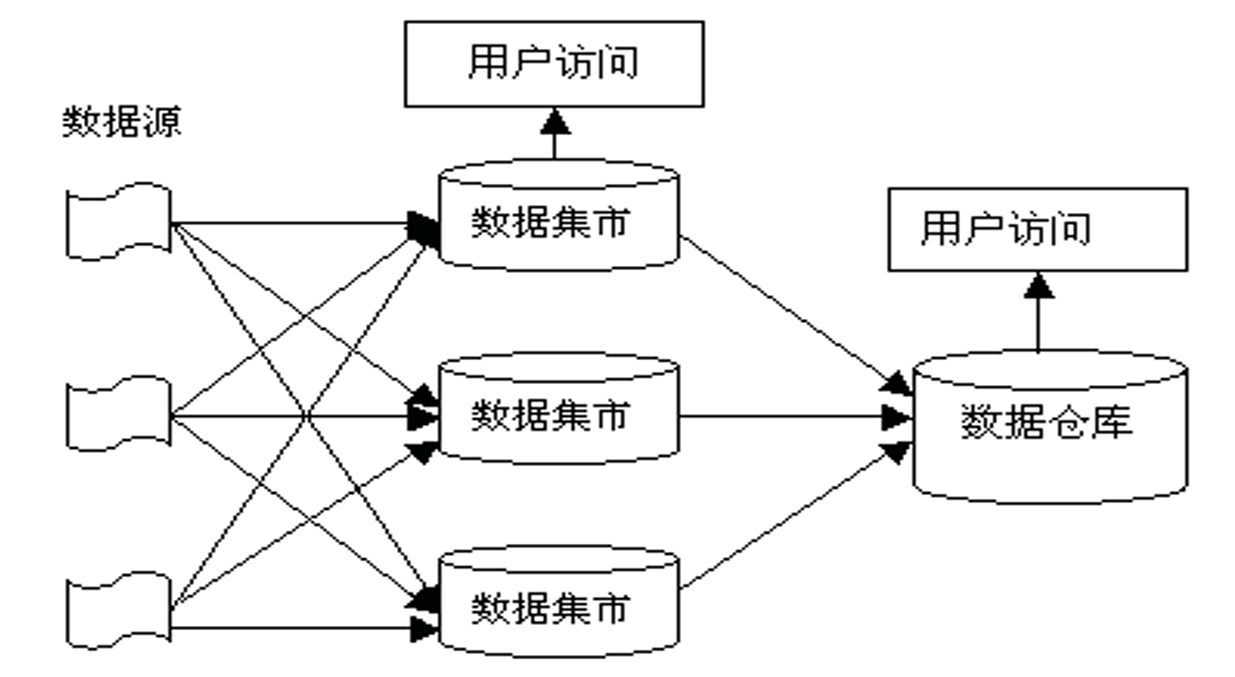
\includegraphics[width=0.97\linewidth]{images/自底向上的结构.png}
	\end{minipage}
	}

    \subfloat[总线结构的数据集市]{
	\begin{minipage}[t]{0.58\linewidth}
	\centering
	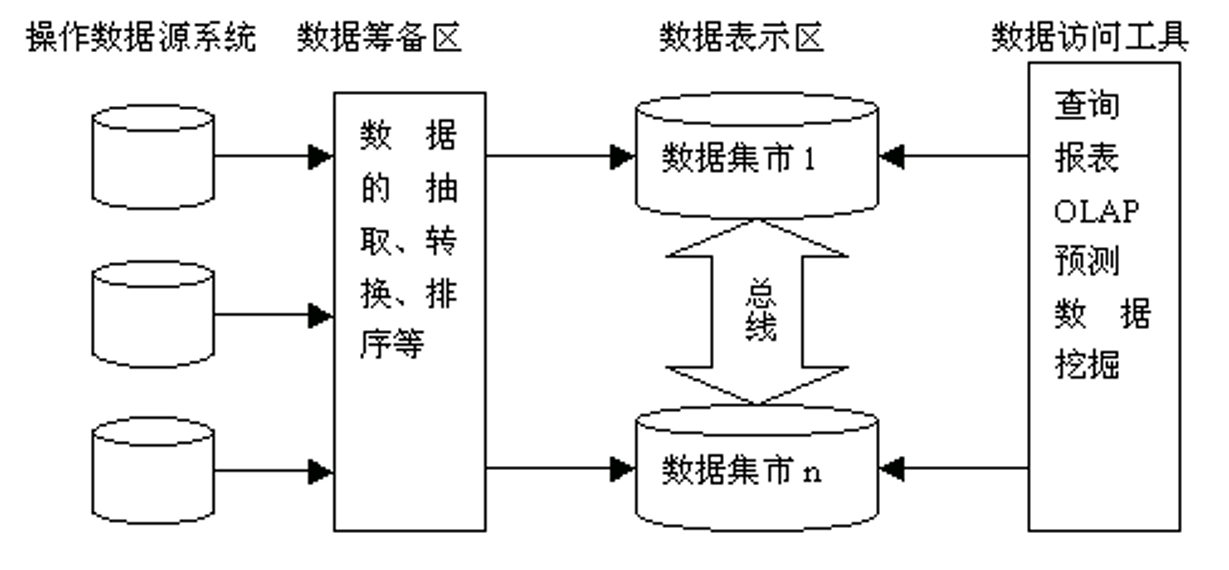
\includegraphics[width=0.97\linewidth]{images/总线结构的数据集市.png}
	\end{minipage}
	}
	\subfloat[企业级数据集市结构]{
	\begin{minipage}[t]{0.38\linewidth}
	\centering
	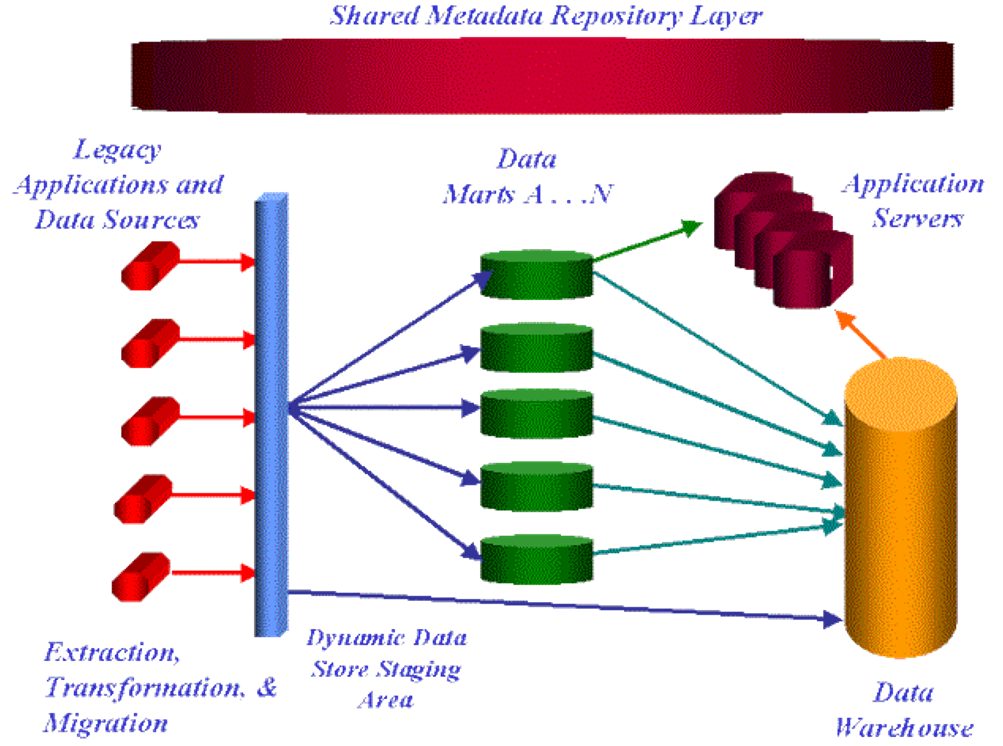
\includegraphics[width=0.97\linewidth]{images/企业级数据集市结构.png}
	\end{minipage}
	}
	\centering
	\vspace{-1.5em}
\end{figure}

\begin{spacing}{1.2}
    \centering
    \begin{longtable}{|m{1.2cm}<{\centering}|m{5cm}|m{4.4cm}|m{3.5cm}|}
        \hline
        方法        & \multicolumn{1}{c|}{数据仓库与数据集市的关系}                                                                     & \multicolumn{1}{c|}{优点}                                & \multicolumn{1}{c|}{缺点}                          \\ \hline
        自顶向下的结构   & {\kaishu 构建企业数据仓库}:公共中央数据模型;数据再加工;减少冗余和不一致性;搜集历史的、细节的、全局的数据。{\kaishu 基于企业数据仓库构建数据集市}:选定企业模型下的部门主题;聚集数据;建立集市数据对企业数据仓库的依赖关系 & 建立数据集市能够减轻DW访问负载;各部门可以任意处理数据;数据转换和整合在DW阶段统一完成;具备数据缓冲功能 & 成本高、见效慢、数据集市间不共享资源                               \\ \hline
        自底向上的结构   & {\kaishu 构建数据集市}:划定主题区域;快速实施本地自治;易于复制;数据再加工;允许一定的冗余和不一致。{\kaishu 基于数据集市构建企业数据仓库}:确定各数据集市的可用性;模型的合并;消除不同数据集市之间的数据不一致性      & 见效快、启动资金少                                              & 各个部门都要进行数据清理整合;可能造成“蜘蛛网”、数据不一致等问题;总体上没有节约资金      \\ \hline
        总线结构的数据集市 & 不建立数据仓库而直接建立数据集市;各个数据集市不是孤立的,相互之间通过一种共享维表和事实表的“总线结构”紧密联系在一起                                           & 共享维表和事实表,解决了建立数据集市的许多问题                                & 这种结构基于多维模型,应用限制于OLAP;多个数据源直接影响多个集市,造成数据仓库结构不十分稳定 \\ \hline
        企业级数据集市结构 & 在没有数据仓库的前提下用总线结构构建数据集市                                                                                & 数据集市遵循总线结构进行独立开发部署                                     & ETL过程不存在数据结构问题                                   \\ \hline
    \end{longtable}
\end{spacing}
\vspace{-0.5em}

\end{solution}


\begin{problem}
\ding{172} 请给出一个具体的数据立方体模型的例子。(绘图说明)

\ding{173} 以该数据立方体为例介绍 OLAP 中的维和层的概念。

\ding{174} 以该数据库立方体中的某一维为例,举例说明什么是切片 (slice),切块 (dice)、数据概括 (roll-up) 和数据细化 (drill-down) 操作。
\end{problem}

\begin{solution}
\begin{figure}[H]
    \centering
    \vspace{-0.2em}
    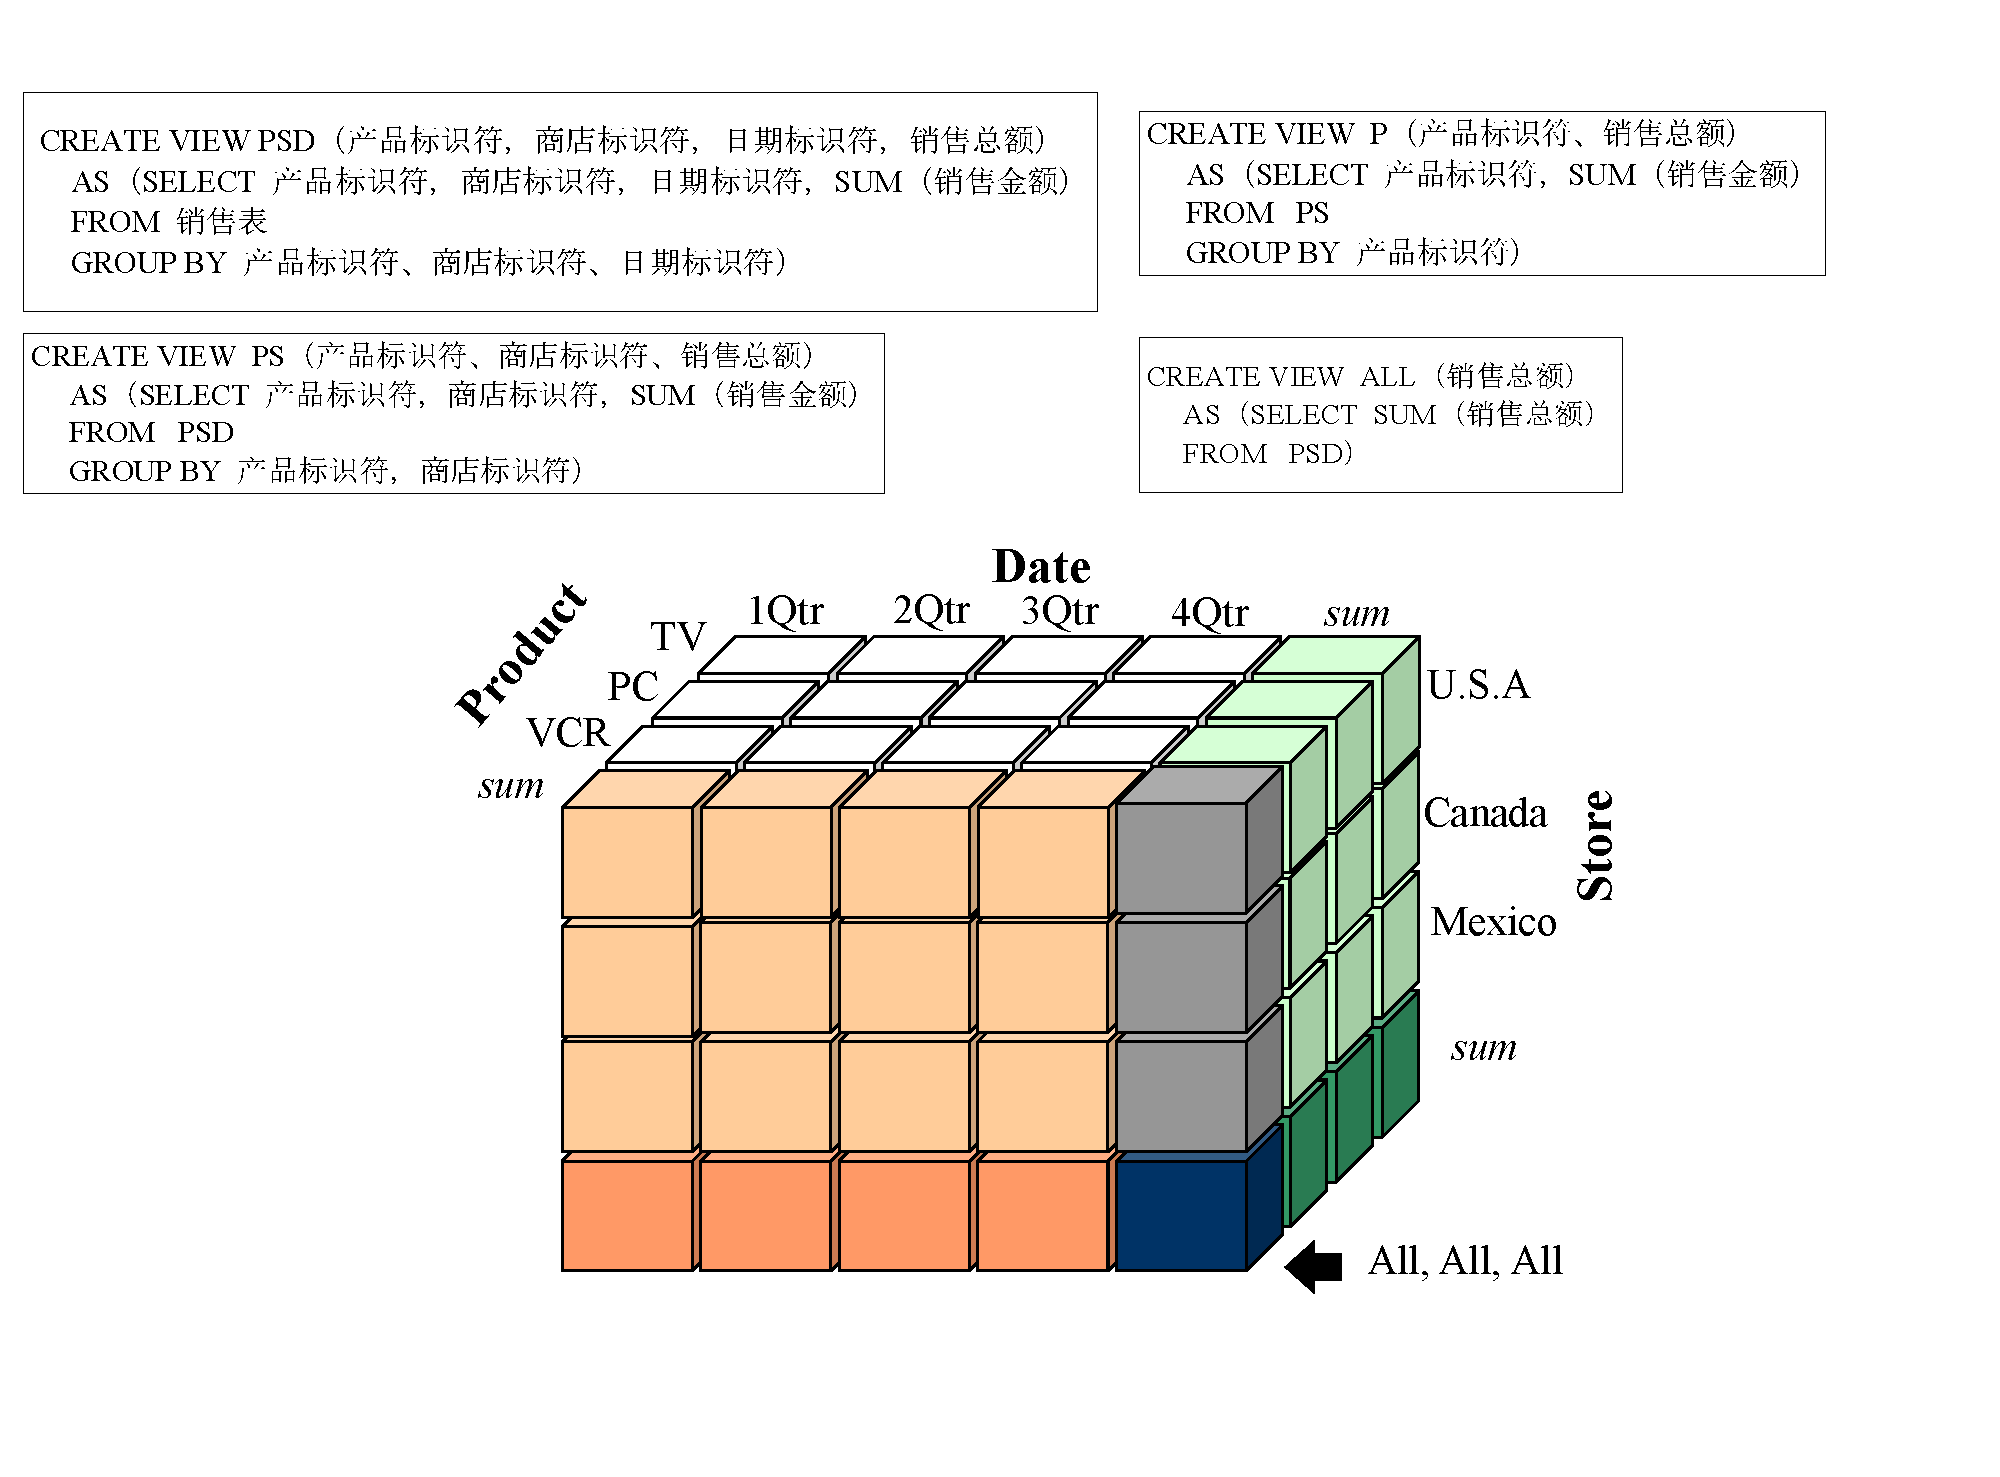
\includegraphics[width=0.95\textwidth]{images/数据立方体.pdf}
    \caption*{数据立方体模型示例}
    \vspace{-1em}
\end{figure}

维(Dimension):观察度量值的角度
\begin{itemize}
    \item 例如可以从三个“维”角度观察“销售金额”这个对象
    \begin{itemize}
        \item 时间维:可从时间角度统计(所有)商品在不同时间段内的销售(总)金额,以便于分析其与时间之间的关系
        \item 商品维:根据商品的分类情况统计每一类商品的销售金额,以便于分析其与商品类型之间的关系
        \item 地域维:可根据每个连锁店所在的地域统计其销售(总)金额,以便于分析其与地域之间的关系
    \end{itemize}
\end{itemize}

层(Layer):在分析型应用中,对分析对象可以在不同的深度层面上进行分析与观察,并可能得到不同的分析结果。因此,“层”反映了对分析对象的观察深度。(可以使维度的取值有不同的度量)
\begin{itemize}
    \item 按如下的方法进行层次划分
    \begin{itemize}
        \item 按商品的价格分为:高档,中档,低档
        \item 按商品的供应商分为:外资,合资,国营,私营,个体
        \item 按购买商品的顾客信息
        \item 按照年龄层次来划分:老年,中年,青年,少年儿童,婴儿
        \item 按照所从事的职业来划分……
    \end{itemize}
\end{itemize}

维成员:维的一个取值称为该维的一个“维成员”

数据单元(单元格):当多维数组的每一维都选中一个维成员,这些维成员的组合就唯一确定了一个观察对象的值,即\ (维成员1,维成员2,$\cdots$,维成员$n$,对象值),这样一个值或存放该值的地方称为一个“数据单元”

\begin{figure}[H]
	\setcounter{subfigure}{0}
	\centering
	\vspace{-1em}	
	\subfloat[切片]{
	\begin{minipage}[t]{0.48\linewidth}
	\centering
	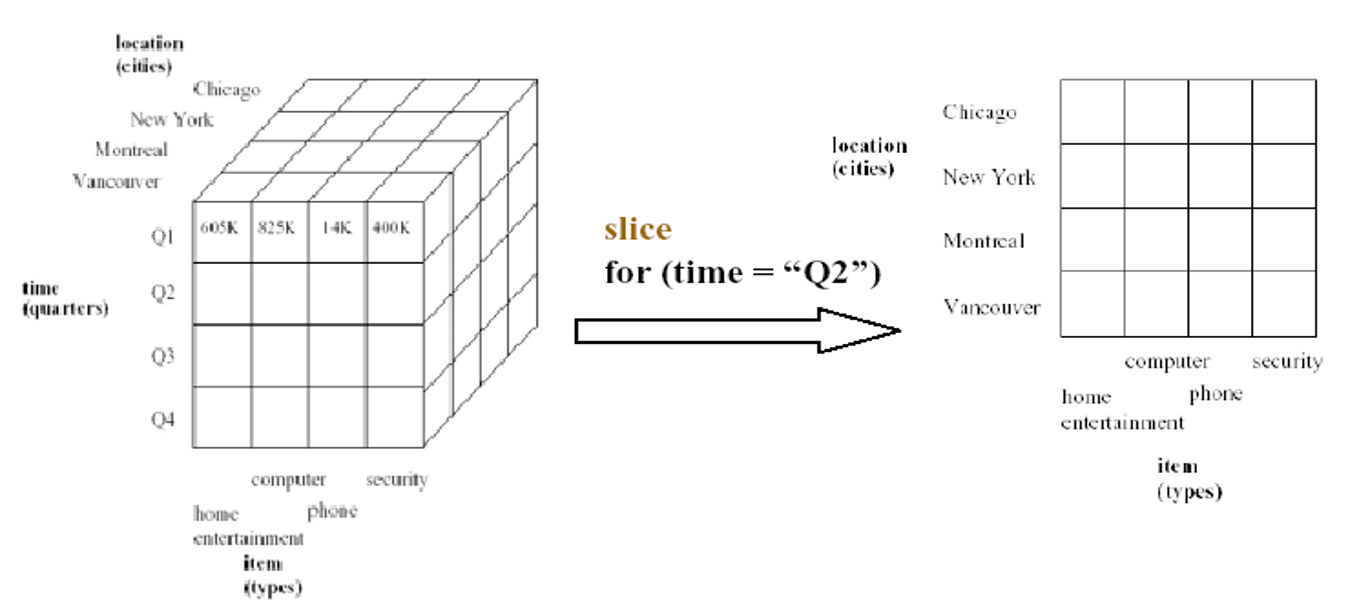
\includegraphics[width=0.97\linewidth]{images/切片.png}
	\end{minipage}
	}
	\subfloat[切块]{
	\begin{minipage}[t]{0.48\linewidth}
	\centering
	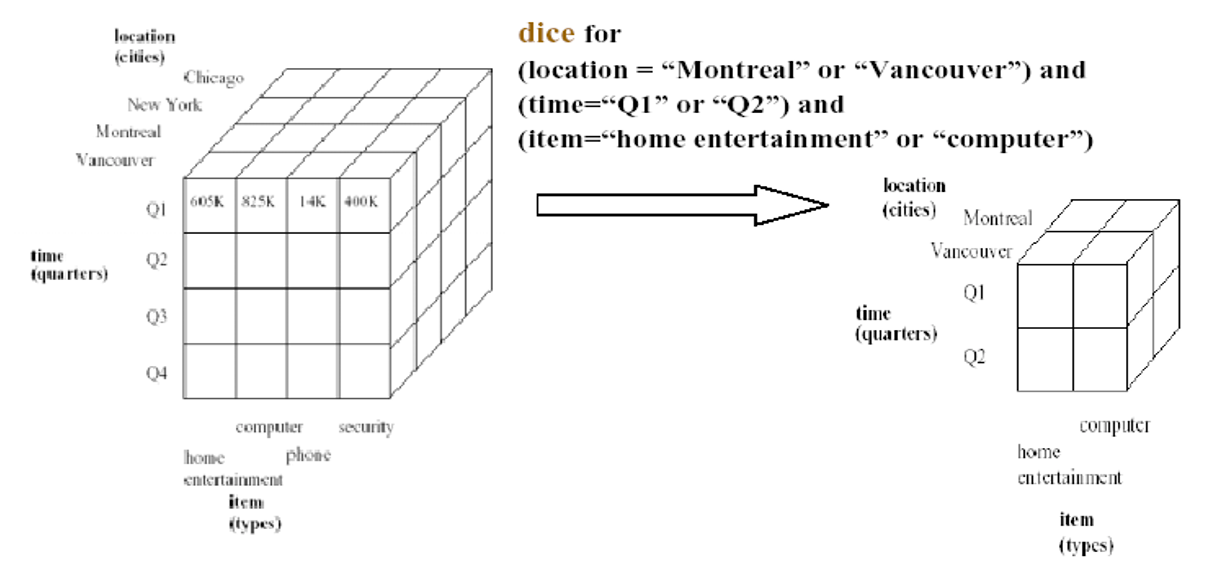
\includegraphics[width=0.97\linewidth]{images/切块.png}
	\end{minipage}
	}

	\subfloat[上钻]{
	\begin{minipage}[t]{0.48\linewidth}
	\centering
	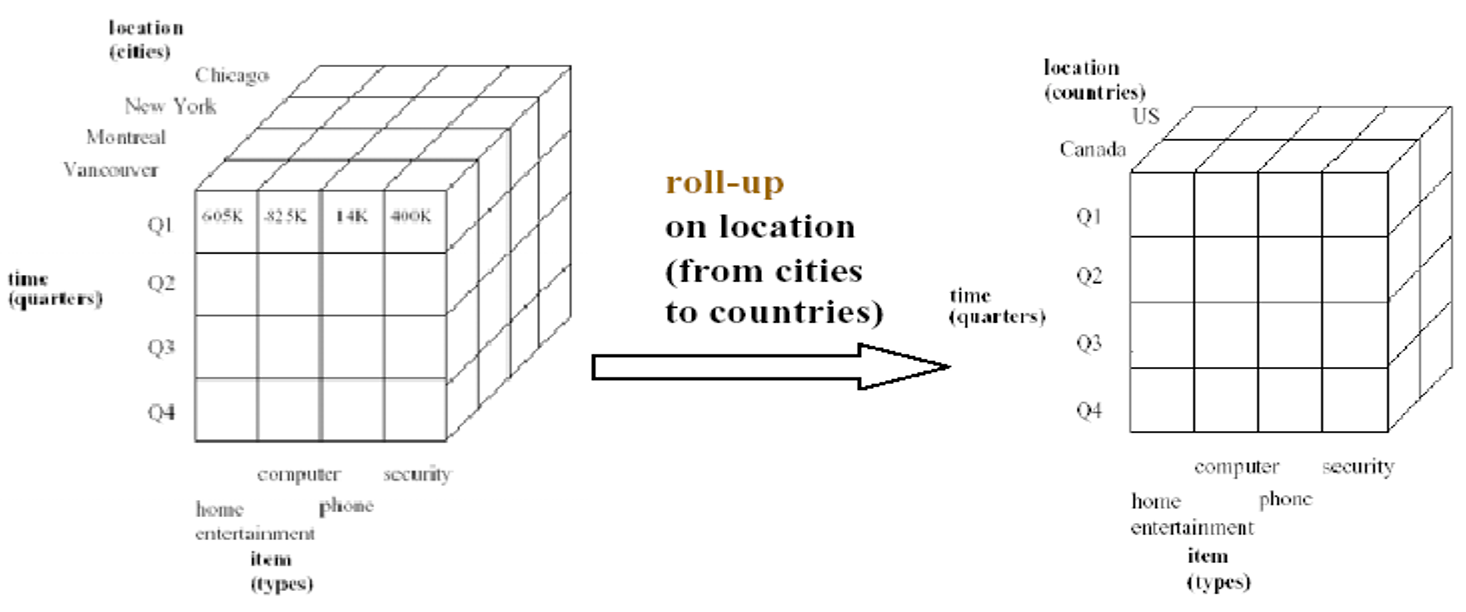
\includegraphics[width=0.97\linewidth]{images/上钻.png}
	\end{minipage}
	}
    \subfloat[下钻]{
	\begin{minipage}[t]{0.48\linewidth}
	\centering
	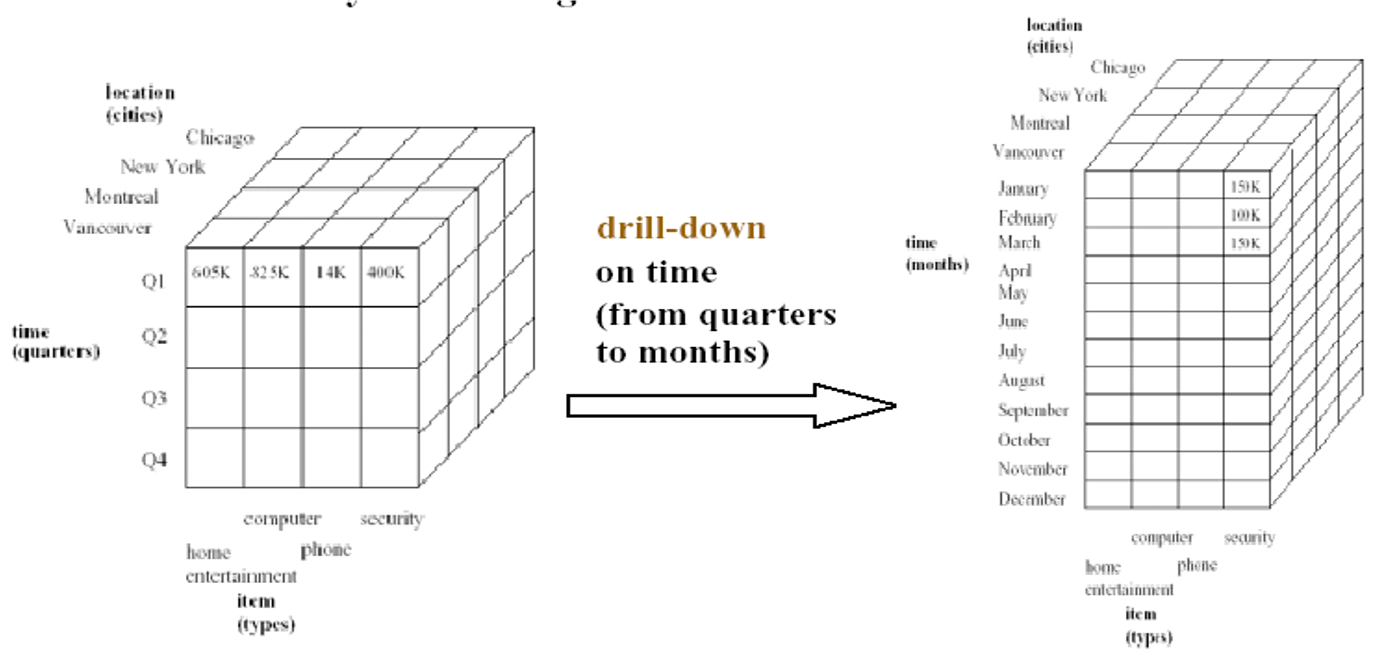
\includegraphics[width=0.97\linewidth]{images/下钻.png}
	\end{minipage}
	}
	\centering
	\vspace{-1.5em}
\end{figure}

\begin{wraptable}{r}{6.9cm}
    \centering
    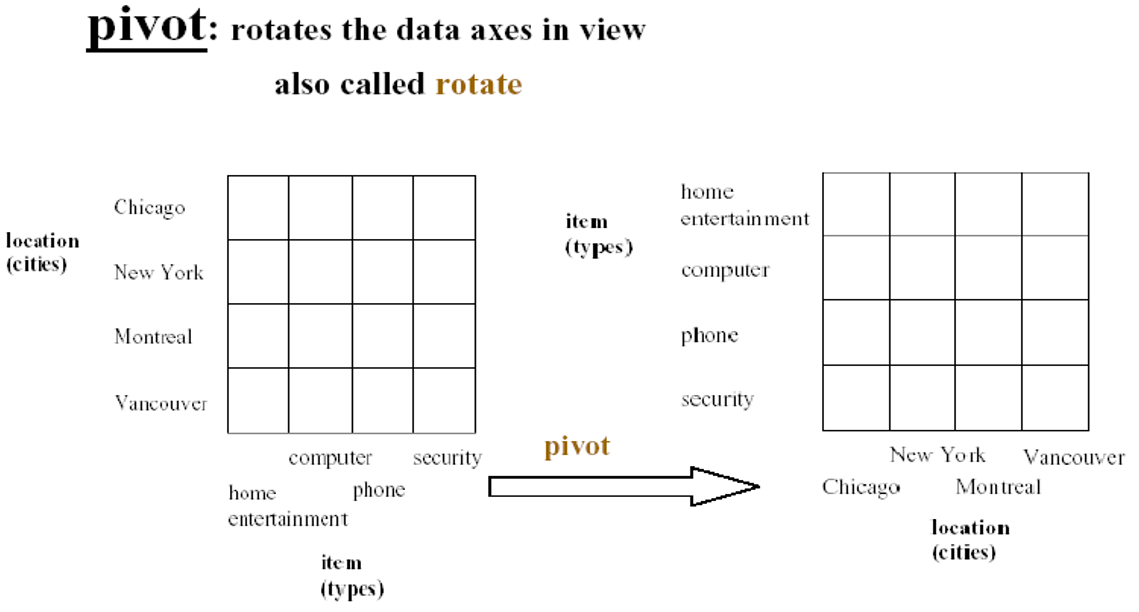
\includegraphics[width=6.8cm]{images/旋转.png}
    \caption*{旋转}
    \vspace{-3em}
\end{wraptable}
$\bullet$切片(Slice):根据某一维上的某个维成员值选择统计数据进行分析

$\bullet$切块(Dice):根据某一维上的某个维成员取值的区间选择统计数据进行分析;根据多个维度上的维成员取值的区间选择统计数据进行分析

$\bullet$上钻/数据概括(roll up):将多维下标的取值提升到较高的概念层次上,从而形成新的统计查询结果,并进行分析

$\bullet$下钻/数据细化(drill down):将多维下标的取值降低到较低的概念层次上,从而形成更细致的统计查询结果,并进行分析

$\bullet$旋转(Pivot/Rotate):调整维的排列次序的动作称为旋转

$\bullet$跨钻(drill across):对多个事实进行操作

$\bullet$钻透(drill through):下钻至数据立方体的最低细节后,继续细化至数据仓库/数据库的关系型表格
\end{solution}

\begin{problem}
现有销售事实表及其隶属的维度定义如下,其中客户维度和销售事实之间采用自然关键宇进行连接。

假设某一特定客户元组的初始状态为
\begin{table}[H]
    \centering
    \vspace{-0.5em}
    {\kaishu \begin{tabular}{ccccc}
    客户编号 & 姓名 & 地址   & 购买金额总和 & 上次购买日期   \\
    001  & 张三 & 明湖小区 & 1000   & 2008-1-3
    \end{tabular}}
    \vspace{-1.5em}
\end{table}

\begin{wraptable}{r}{6.5cm}
    \centering
    \vspace{-1.5em}
    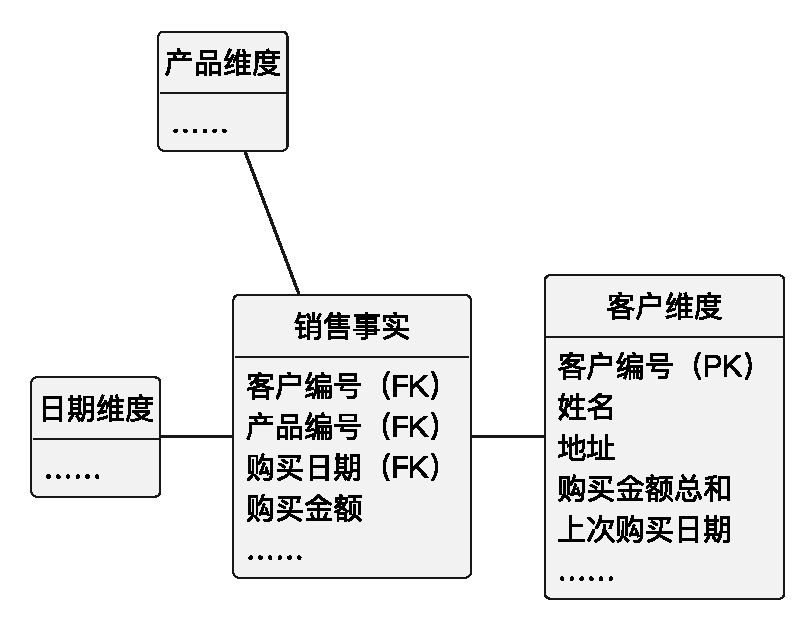
\includegraphics[width=6cm]{images/销售事实表及其隶属的维度定义.eps}
\end{wraptable}

该客户分别于
\vspace{-0.7em}
\begin{center}
2008-2-1 花费200元\ 购买了编号为 P003 的产品\\
2008-3-5 花费300元\ 购买了编号为 P002 的产品\\
2008-5-1 花费100元\ 购买了编号为 P00S 的产品\\
2008-8-2 花费400元\ 购买了编号为 P007 的产品\\
\end{center}
\vspace{-0.7em}
\ding{172} 试以该过程为例,解释为何采用自然关键字进行连接的事实表和维度表体系会影响数据仓库的历史完整性,并解释为何数据仓库的历史完整性会影响到分析性数据环境中的分析性应用。

\ding{173} 试以该过程为例,分别解释如何采用类型1,类型2,类型3和类型6四种方法,对客户维度进行处理。需给出对应的数据结构,和对应的数据演化过程。

\end{problem}

\begin{solution}

\end{solution}

